\chapter{提案手法}
\label{method}
本章では提案手法の詳細を述べる.

\section{概要}
本研究はヘルメットをキーの代わりとして用いることを目標とし,利用者が圧力センサを搭載したヘルメットを装着して,頭部形状を取得することで,本人認証を行う手法を提案する.提案するシステムの構成を図\ref{system}に示す.ヘルメットの内側には32個の圧力センサが搭載されており,1回のサンプリングで32次元のデータを取得する.提案するシステムでは,あらかじめ学習フェーズとして,二輪車の所有者など認証したいユーザの頭部の32次元の圧力センサデータを,ヘルメットを複数回装着することで収集しておく.そして,識別フェーズでは,ヘルメットを装着した人物の32次元の圧力センサデータと事前に収集した学習データの距離を計算し,距離が閾値以下であれば本人であると認証する.

\section{登録データとの距離計算}
学習データと入力データの距離計算方法として,マハラノビス距離を用いる.マハラノビス距離とは多変数間の距離計算手法のひとつであり,データの分布を考慮して正規化した距離を計算できる.学習データを$\bm{x}_i~(i=1,\dots, m)$,認証するユーザの入力データを$\bm{y}$とする.ただし,$m$は学習データの個数である.
学習データの平均値ベクトル$\bm{\mu}$と分散共分散行列$\bm{\Sigma}$を次式で求める.
\begin{eqnarray}
  \bm{\mu} &=& \frac{1}{m}\sum_{i=1}^{m}\bm{x}_i \\
  \bm{\Sigma} &=& \frac{1}{m}\sum_{i=1}^{m}(\bm{x}_i-\bm{\mu})(\bm{x}_i-\bm{\mu})^T
\end{eqnarray}
このとき,入力データが事前に登録された本人のデータであれば,学習データ$\bm{x}_i$と入力データ$\bm{y}$は同じ分散共分散行列$\bm{\Sigma}$の確率分布に従うため,学習データ$\bm{x}_i$と入力データ$\bm{y}$のマハラノビス距離は
\begin{eqnarray}
  d(\bm{y},\bm{x}_i) = \sqrt{(\bm{y}-\bm{x}_i)^{T}\bm{\Sigma}^{-1}(\bm{y}-\bm{x}_i)}
\end{eqnarray}
と定義できる.

\section{認証判定}
閾値を$\theta$とおき,
\[
  \theta < min_i(d(\bm{y},\bm{x}_i))~(i=1,\dots,m)
\]
を満たす場合,入力データ$\bm{y}$は所有者以外の他人から得られた頭部データであると判定し拒否する.
一方で,
\[
  \theta \geq min_i(d(\bm{y},\bm{x}_i))~(i=1,\dots,m)
\]
を満たす場合,入力データ$\bm{y}$は所有者本人から得られた頭部データであると判定し認証する.

\begin{figure}[!t]
  \centering
    \includegraphics[width=1\linewidth]{figure/system.eps}
  \caption{システム構成}
  \label{system}
\end{figure}